\documentclass[UTF8]{ctexart}
\usepackage{graphicx}
\usepackage{float}
\usepackage{ragged2e}
\usepackage{amsthm}
\usepackage{amssymb}
\usepackage{amsmath}
\usepackage{wrapfig}
\title{暗物质和暗能量}
\author{limbo137}
\begin{document}
\maketitle
\tableofcontents
\section{什么是暗物质}
\subsection{从旋转曲线说起}
宇宙中有各种各样的星系(galaxies),我们所在的银河系(Galaxy)是其中一个。星系的共同特征是围绕一根中心轴旋转。各星体旋转的切向速度$v$,或者说角速度$\omega=\frac{v}{r}$,是旋转半径r的函数,函数$v(r)$和$\omega(r)$的函数形式与质量分布有关,星体的速度$v$是通过多普勒效应来观测的,把观测到的数据绘制成$v(r)$曲线,叫做星系的\textbf{旋转曲线(rotation curve)}。将实测的旋转曲线与不同的理论模型相比较,可以获得星系中质量分布的一些信息。星系一般是扁平的,但有许多迹象表明,它们的外面常常有一个近似球形的暗物质晕。
\begin{figure}[H]
    \centering
    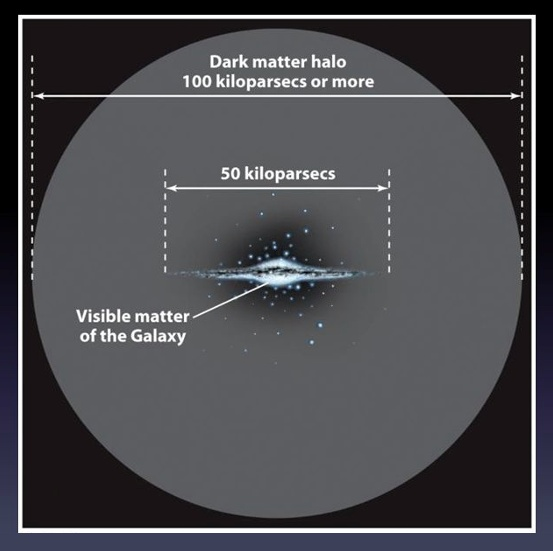
\includegraphics[width=6cm]{v2-0eb8fd5dd031f31c2e089a84ae1fab85.jpg}
    \caption{星系被暗物质晕所包绕}
    \label{fig:my_label}
\end{figure}

%我们可以先讨论一些简单模型的旋转曲线,例如我们考虑一个旋转中的半径为$R$的均匀球状星系,那么根据万有引力定律
%我们可以选取转动参考系,在球内,有\[\frac{\mathrm{d}^2r}{\mathrm{d}t^2}-\omega^2r=-\frac{GM}{r^2}\]
%其中$M$为以$r$为半径球的内部质量,由于是均匀球体,我们可以得到
%\[M=\frac{4\pi \rho r^3}{3}\]
%结合上两式,有
%\[\frac{\mathrm{d}^2r}{\mathrm{d}t^2}-\omega^2r=-\frac{4\pi G \rho r}{3}\]
%由于是稳定结构,故径向加速度为0,有
%\[\omega^2=\frac{4\pi G \rho }{3}\]
%可以看到此时$\omega$与$r$无关,只与密度有关,也就是说,整个星系都在以同一角速度旋转。

%在球外分布的星体同理,此时$M$为常数
%\[M=\frac{4\pi  \rho R^3}{3}\]
%于是
%\[\frac{\mathrm{d}^2r}{\mathrm{d}t^2}-\omega^2r=-\frac{4\pi G \rho R^3}{3r^2}\]
%进而得到开普勒第三定律
%\[\omega=\sqrt{\frac{4\pi G \rho R^3}{3}}r^{-\frac32}\]
%可以看出距离星系中心越远的地方,转动的角速度越慢

一般的星系都是扁平状的,根据牛顿的引力理论,其旋转曲线在$r$较小的时候应该正比于$r$,在$r$较大的时候应该正比于$r^{-\frac12}$,但是,
在1933年,瑞士天文学家Fritz Zwicky将理论结果与实际观测相比较时,却发现相去甚远(如图2,其中A线为理论预测,B线为实际观测)
\begin{figure}[H]
    \centering
    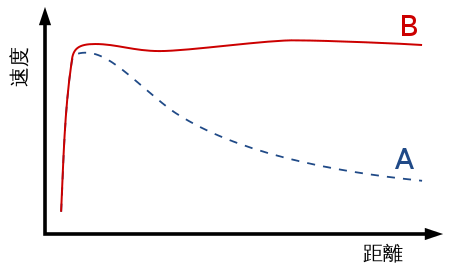
\includegraphics[width=9cm]{langzh-450px-GalacticRotation2.svg.png}
    \caption{旋转曲线的理论值和实验值}
    \label{fig:my_label}
\end{figure}

几乎所有来自地外的宇宙信息都是通过光子来传播的,但并非宇宙间的物质都发光,其实恰恰相反,由图可以看出,直到观测的最远点,实测曲线仍没有下降的趋势,这说明,星系中的\textbf{暗物质(dark matter)},不但很多,而且延伸到很远。我们尚没有办法估计,暗物质的质量在星系中占多少比例,人们普遍的看法是,星系中90\%到99\%的物质都是暗的。如果星系中的所有物质都发光,明亮的星系要比现在现在大几十倍,用肉眼看去,将会有上千个冕光大如明月的星系浮现在璀璨的星空。

\subsection{暗物质的证据}
\subsubsection{引力透镜}
引力透镜源于光在引力作用下的偏折,根据著名的广义相对论,引力是时空弯曲的结果,这样的弯曲会使光线偏折,这一现象在1919年被首次观测到,之后在光学望远镜下也观察到了很多这样的现象(图3),我们称之为\textbf{引力透镜(Gravitational Lens)}。
\begin{figure}[H]
    \centering
    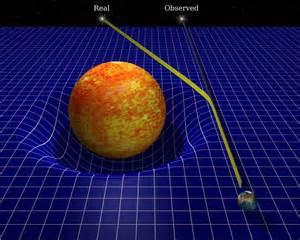
\includegraphics[width=6cm]{cf7afb5a65d8442d71a7c7db51836b04.jpg}
    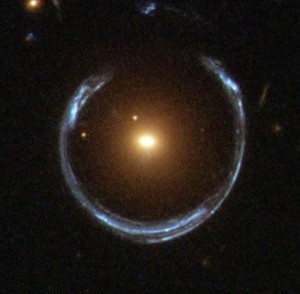
\includegraphics[width=5cm]{db70e090804d296d47be7aef28127faa.jpg}
    \caption{(左)时空弯曲导致的光线偏折(右)大质量天体将其后面的星系发出的光畸变为一个圆环}
    \label{fig:my_label}
\end{figure}


通过对引力透镜效应的研究,我们可以测算出这些暗物质的具体分布,甚至做出3D模型
\begin{figure}[H]
    \centering
    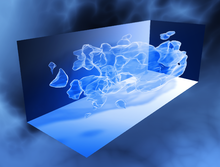
\includegraphics[width=8cm]{220px-COSMOS_3D_dark_matter_map(1).png}
    \caption{暗物质大规模分布的3D映射图}
    \label{fig:my_label}
\end{figure}
\subsubsection{子弹星团}
引力透镜是目前最好的观测暗物质的方式,通过引力透镜观测到的一个非常显著的例子就是子弹星团(Bullet Cluster)

蓝色代表暗物质分布,红色是通过X射线观测到的星系团中气体的分布。可以发现,这个星系团实际上是两个星系团正在进行并合的产物。气体在并合过程中由于相互作用,互相穿过对方以后,已经完全变形了。而不发光的暗物质则表现的完全不同,两团物质依然十分分明,碰撞过后对形态并没有什么影响。因此可以发现,暗物质之间的相互作用比正常物质要弱的多。
\begin{figure}[H]
    \centering
    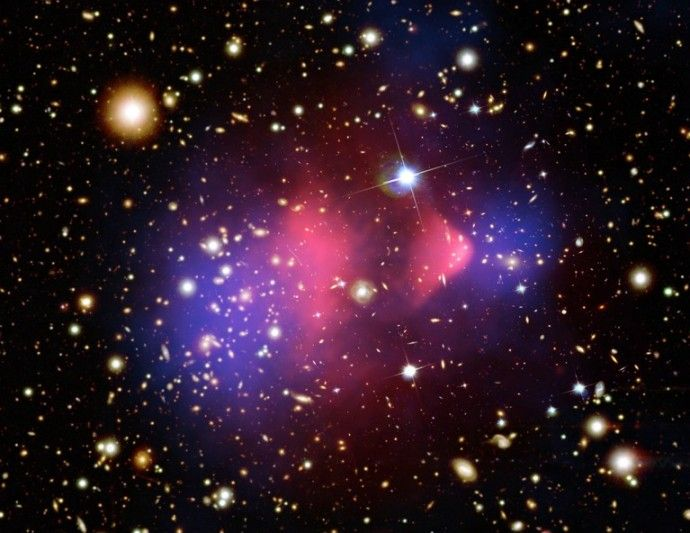
\includegraphics[width=6cm]{8724e7ea8d9cd44483aa93287bae4158_1440w.jpg}
    \caption{子弹星团中的暗物质}
    \label{fig:my_label}
\end{figure}

上述的暗物质的观测证据有三个局限性:①证据都是星系团尺度上的,我们需要更大尺度上的证据;②不能告诉我们早期宇宙中是否存在暗物质(
因为星系团最早也要形成于宇宙诞生十亿年后
);③难以精确地告诉我们暗物质具体有多少。
宇宙微波背景辐射(CMB)温度各向异性
的测量可以扫除以上的局限性。
\subsubsection{宇宙微波背景辐射}
我们可能常常认为宇宙的真空中“一无所有”,其实,通过射电望远镜,我们可以发现一个微弱的辐射,称为\textbf{宇宙微波背景辐射(Cosmic Microwave Background Radiation)},由美国的两位射电天文学家Arno Penzias和Robert Wilson于1965年偶然发现,他们也在1978年因这项发现获得诺贝尔物理学奖。我们正泡在这样的辐射汤中,这个辐射很微弱但无处不在,它是宇宙早期大爆炸后的残余,是宇宙中最古老的辐射。如果将这样的辐射绘制出来,将呈现出宇宙在婴儿时期的样子(图5上)


CMB是大爆炸理论的有力依据。2001年6月,美国宇航局发射了第二个CMB太空任务,Wilkinson各向异性探测(Wilkinson Microwave Anisotropy Probe),以更精确地测量全天空上的大规模各向异性(图5下)。虽然暗物质和普通物质都是物质,但它们的行为方式并不相同。特别是在早期的宇宙中,普通物质被电离,通过汤姆森散射与辐射强烈地相互作用。暗物质不直接与辐射相互作用,但它的引力势(主要是大尺度上)及其对普通物质密度和速度的影响CMB。因此,普通和暗物质扰动会随着时间的不同而变化,在宇宙微波背景(CMB)上留下不同的印记。
\begin{figure}[H]
    \centering
    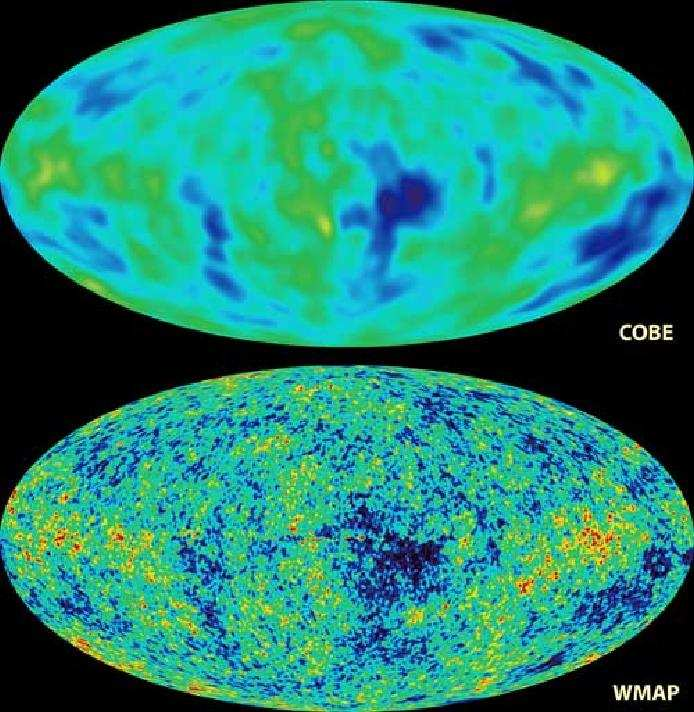
\includegraphics[width=8cm]{cmb.png}
    \caption{宇宙微波背景(CMB)和Wilkinson各向异性探测(WMAP)}
    \label{fig:my_label}
\end{figure}

CMB包含着早期宇宙的物理信息。当前的Planck卫星实验可以精确地测量CMB的温度各向异性谱,如下图所示。可以看到它存在三个非常明显的峰,其中从左到右第二、三个峰和暗物质密切相关。
\begin{figure}[H]
    \centering
    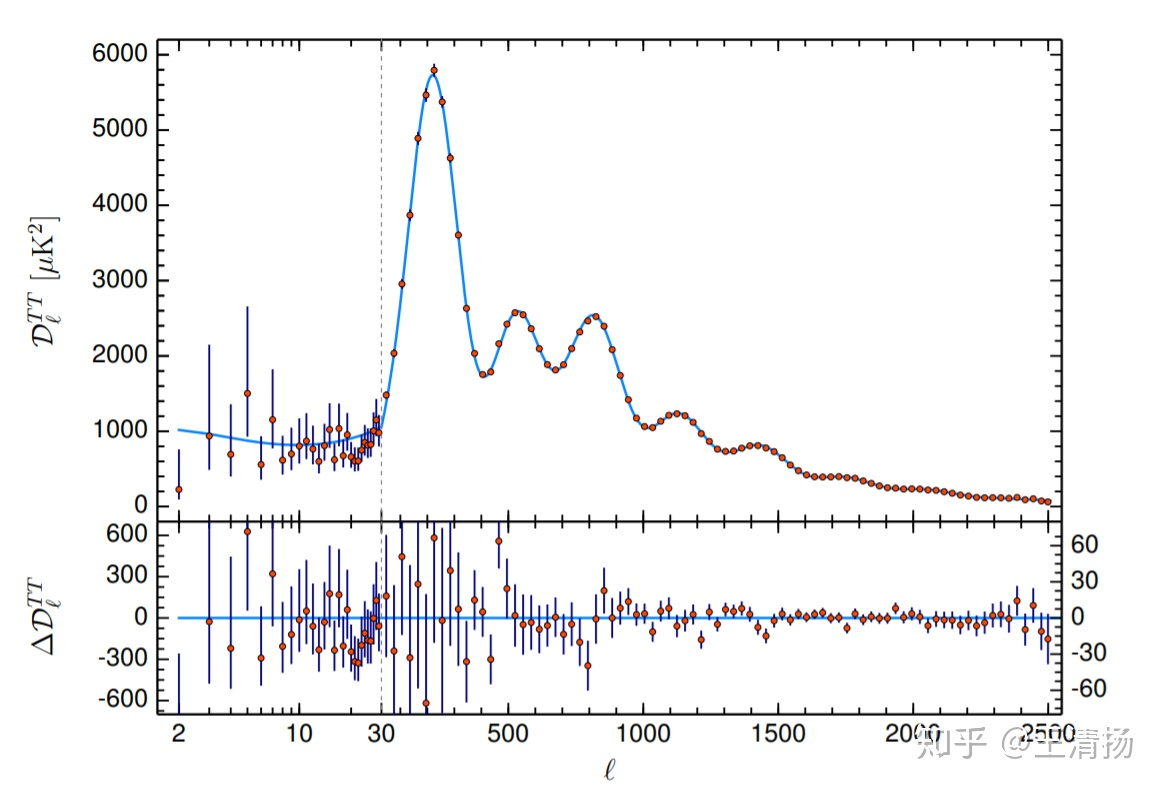
\includegraphics[width=8cm]{v2-fb241b2c22ab2142b5acb5c980928200.jpg}
    \caption{CMB的温度各向异性谱}
    \label{fig:my_label}
\end{figure}
第一个主峰包含了宇宙几何、年龄的信息;第二个峰来自于重子声学振荡,它告诉我们宇宙中可见物质有多少;第三个峰与第二个峰的高度差决定了可见物质与暗物质的比例。
由此可以推出宇宙中可见物质的比重是4.9\%,暗物质的比例是26.2\%(剩下68.9\%是暗能量)。做一个总结:
CMB温度各向异性谱的测量可以确定暗物质在宇宙诞生初期就已存在(因为CMB形成于宇宙诞生38万年时),且可以确定今天暗物质在宇宙中的比重是26.2\%
\begin{figure}[H]
    \centering
    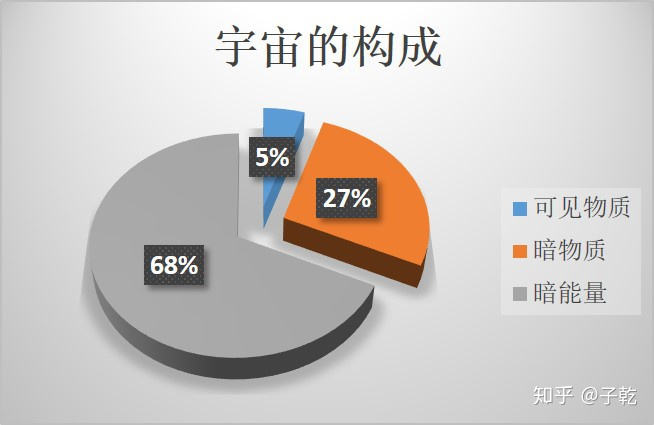
\includegraphics[width=8cm]{v2-cb275465102b39d2d2821a162e56b829.jpg}
    \caption{宇宙的组成成分}
    \label{fig:my_label}
\end{figure}
\subsection{候选者动物园}

在讨论暗物质可能是什么之前,我们必须对暗物质的特性进行简要地总结,主要有以下几点:


1.暗物质必须在早期宇宙中产生。这是CMB的观测结果要求的。

2.暗物质必须是稳定的。因为暗物质产生后经过了138亿年的演化依然保有足够大的丰度。

3.不参与电磁相互作用,或者说不带电荷。因为观测表明暗物质不与光子发生相互作用。

4.不参与强相互作用,或者说不带色荷。因为如果暗物质是强子的话,稳定性会要求它的质量非常小以至于不能衰变到其他强子(大质量的强子寿命非常短)。然而在粒子对撞机中没有发现过这么轻的强子。

5.暗物质主要是非相对论性的(速度远小于光速),即冷暗物质(CDM).

我们会列出一些主流的猜想来解释暗物质,大多是一些粒子,这些粒子千奇百怪,故有动物园(zoo)一称,我们通常称质子和中子这种构成常见物质的粒子称为\textbf{重子(Baryon)},上文中已经讨论过暗物质应该不是由重子构成的,所有我们有一些其他的非重子的候选\\
1.中微子

中微子(neutrinos)一直被认为是极好的候选,原因十分简单,因为他们已经被证实是确实存在的,然而遗憾的是,目前我们仍然不能确定中微子是否有质量,即使有,其质量也存在一个上限,通过计算可知,它还远远不及暗物质的质量,但是目前是否存在其它机制使得中微子突破这个质量上限,还有待进一步论证。\\
2.引力微子

引力微子(Gravitinos)是引力子(Graviton)在超对称下的的超伴子,引力微子可以是最轻的超对称粒子而且是最稳定的,因此引力微子在理论上有很强的动机。但这种粒子非常难观测到\\
3.轴子

\textbf{轴子(Axions)}也是热门的候选人之一,轴子的发现是为了解决CP不对称的问题,它们与普通粒子之间的相互作用非常微弱,也是目前的一个研究方向。\\
4.原初黑洞

暗物质的候选也可能是某种天体,例如\textbf{原初黑洞}宇宙在诞生$10^{-30}$秒内经历了一场暴胀过程。暴胀会产生原初密度扰动,而如果某个区域的扰动幅度足够大,它就可以坍缩形成原初黑洞。虽然目前人们并没有发现原初黑洞,但这不妨碍理论上的讨论。由于霍金辐射效应,原初黑洞从诞生后会慢慢蒸发损失质量,但黑洞质量越大蒸发速度越慢,因此计算可知质量大于$10^{15}$克的原初黑洞可以存活到今天充当暗物质。\\
5.Kaluza-Klein观点

Kaluza-Klein理论是历史上对同一电磁力和引力的一次重要尝试,这个理论假设了第五维时空,而在这种时空下,电磁学方程会自然而然的产生,虽然没有考虑到强弱相互作用(当时并没有发现),但为后来的很多理论例如弦论(string theory)提供了重要思路。在其假设的第五维度中,也提出了一种暗物质候选者,一种具有右手中微子的规范量子数的奇异粒子\\
6.镜像物质

1956年李政道和杨振宁发现了弱相互作用中宇称(parity)对称性被破坏,宇称不守恒的意义是极其深刻的,现代物理对这一现象的理解还远远不够。下面要介绍的镜像世界模型就是对宇称不守恒的一个自然的拓展。三个前苏联物理学家(Kobzarev, Okun, Pomeranchuk)首先在1966年提出了镜像粒子(mirror particles)的可能存在。他们的灵感来自于当时刚刚发现的CP对称破坏的发现,他们提出镜像粒子和我们世界里的普通粒子(ordinary particles)几乎一样,但是它们参与它们自己的规范相互作用(几乎就是我们世界的规范相互作用的复制)。除了共享万有引力外,他们猜测,镜像粒子可能通过弱相互作用耦合,但一定非常微弱。新的镜像物质模型也是希望解决暗物质问题的。在新理论中,暗物质就是镜像物质(mirror matter)。而普通和镜像物质之间除引力外不存在其他任何相互作用。这意味着现在几乎所有的暗物质探测项目非常可能都是竹篮打水一场空。镜像物质的讨论非常冷门,目前在这个方向的研究人员很少。
\section{暗物质的探测}
目前探测暗物质的方式主要有三种,我们各举一个例子
\subsection{直接探测}
直接探测实验旨在观察低能反冲,这是由于与暗物质粒子相互作用而引起的,在这种反冲之后,原子核将通过闪烁的光子或声子,并通过敏感的检测设备,从而发出能量。为了有效地做到这一点,保持低背景至关重要,因此此类实验必须在地下深处进行,以减少来自宇宙射线的干扰。中国也建有这样的实验室,位于四川锦屏山地下,
目前,中国锦屏地下实验室有两个暗物质实验项目组,一个是清华大学领导的CDEX(中国暗物质实验)高纯锗暗物质实验,一个是上海交通大学领导的PandaX(熊猫计划)液氙暗物质实验项目。这两个项目组采用的都是直接探测的方法,就是测量暗物质粒子直接碰撞普通物质引起的反冲核的数量和能量。
\subsection{间接探测}
间接探测实验寻找外层空间暗物质粒子湮灭或衰变的产物。例如,在暗物质密度高的区域(例如银河系的中心),两个暗物质粒子可能会湮灭以产生伽马射线或标准模型粒子-反粒子对。如果暗物质粒子不稳定,则它可能会衰减为标准模型(或其他)粒子。这些过程可以通过银河系或其他星系中高密度区域发出的过量伽玛射线、反质子或正电子间接检测出来。我国的“悟空”号目前就在承担这样的任务
\subsection{对撞机搜寻暗物质}
在自然界中探测暗物质粒子的另一种方法是在实验室中制造它们。使用大型强子对撞机(LHC)进行的实验可能能够探测到LHC质子束碰撞产生的暗物质粒子。由于暗物质粒子与普通可见物质之间的相互作用可以忽略不计,如果能探测到其他(不可忽略的)碰撞产物,它可能会以(大量)能量和动量缺失的形式从探测器中被间接探测到。
\section{暗能量}
比起暗物质,人类对\textbf{暗能量(dark energy)}更是知之甚少。我们知道,宇宙中的各部分之间都在通过引力互相吸引,所以如果宇宙在膨胀,那么一定是减速膨胀,然而实验观测往往事与愿违。2011年的诺贝尔奖就表彰了三位天文学家关于宇宙加速膨胀的研究,他们在1998年通过对超新星的观测表明,我们的宇宙在加速膨胀。为了解释这个现象,人们提出应该存在一种暗能量把宇宙“撑开”,而且这种能量应该占宇宙的大部分。

除了超新星观测实验外,还有许多观测实验也表明我们的宇宙中存在暗能量,比如重子声学振荡、宇宙微波背景辐射(CMB)各向异性的测量(前面提到过)等。

暗能量的发现对宇宙学乃至整个物理学的发展有重要意义。从宇宙学的角度讲,暗能量直接决定了宇宙今后的命运,对我们研究晚期宇宙的演化有极其重要的影响。从物理学的角度讲,我们对暗能量这种负压物质的本质一无所知,显然这种物质不同于粒子物理标准模型中的任何一种物质。因此,暗能量涉及到基础物理的根基问题,我们需要想办法加深对它的了解。
\section{宇宙的过去和未来-$\Lambda $CDM理论}
$\Lambda $CDM理论是目前公认比较好的宇宙学模型,即宇宙学常数和冷暗物质模型,所谓冷暗物质,即暗物质的速度远小于光速,在这个模型中,暗物质是星系产生的摇篮,在星系产生过程中将重子物质吸引到一起,使之形成星系等小尺度结构,但暗物质本身却没有这样的小尺度结构,无论是暗物质晕还是其子晕中小尺度结构都是非常不稳定的,因此也不存在暗物质构成的星系和行星。
\end{document}